% Options for packages loaded elsewhere
\PassOptionsToPackage{unicode}{hyperref}
\PassOptionsToPackage{hyphens}{url}
%
\documentclass[
]{article}
\usepackage{amsmath,amssymb}
\usepackage{lmodern}
\usepackage{ifxetex,ifluatex}
\ifnum 0\ifxetex 1\fi\ifluatex 1\fi=0 % if pdftex
  \usepackage[T1]{fontenc}
  \usepackage[utf8]{inputenc}
  \usepackage{textcomp} % provide euro and other symbols
\else % if luatex or xetex
  \usepackage{unicode-math}
  \defaultfontfeatures{Scale=MatchLowercase}
  \defaultfontfeatures[\rmfamily]{Ligatures=TeX,Scale=1}
\fi
% Use upquote if available, for straight quotes in verbatim environments
\IfFileExists{upquote.sty}{\usepackage{upquote}}{}
\IfFileExists{microtype.sty}{% use microtype if available
  \usepackage[]{microtype}
  \UseMicrotypeSet[protrusion]{basicmath} % disable protrusion for tt fonts
}{}
\makeatletter
\@ifundefined{KOMAClassName}{% if non-KOMA class
  \IfFileExists{parskip.sty}{%
    \usepackage{parskip}
  }{% else
    \setlength{\parindent}{0pt}
    \setlength{\parskip}{6pt plus 2pt minus 1pt}}
}{% if KOMA class
  \KOMAoptions{parskip=half}}
\makeatother
\usepackage{xcolor}
\IfFileExists{xurl.sty}{\usepackage{xurl}}{} % add URL line breaks if available
\IfFileExists{bookmark.sty}{\usepackage{bookmark}}{\usepackage{hyperref}}
\hypersetup{
  pdftitle={PDB\_structural\_bioinformatics},
  pdfauthor={Kelly\_F},
  hidelinks,
  pdfcreator={LaTeX via pandoc}}
\urlstyle{same} % disable monospaced font for URLs
\usepackage[margin=1in]{geometry}
\usepackage{color}
\usepackage{fancyvrb}
\newcommand{\VerbBar}{|}
\newcommand{\VERB}{\Verb[commandchars=\\\{\}]}
\DefineVerbatimEnvironment{Highlighting}{Verbatim}{commandchars=\\\{\}}
% Add ',fontsize=\small' for more characters per line
\usepackage{framed}
\definecolor{shadecolor}{RGB}{248,248,248}
\newenvironment{Shaded}{\begin{snugshade}}{\end{snugshade}}
\newcommand{\AlertTok}[1]{\textcolor[rgb]{0.94,0.16,0.16}{#1}}
\newcommand{\AnnotationTok}[1]{\textcolor[rgb]{0.56,0.35,0.01}{\textbf{\textit{#1}}}}
\newcommand{\AttributeTok}[1]{\textcolor[rgb]{0.77,0.63,0.00}{#1}}
\newcommand{\BaseNTok}[1]{\textcolor[rgb]{0.00,0.00,0.81}{#1}}
\newcommand{\BuiltInTok}[1]{#1}
\newcommand{\CharTok}[1]{\textcolor[rgb]{0.31,0.60,0.02}{#1}}
\newcommand{\CommentTok}[1]{\textcolor[rgb]{0.56,0.35,0.01}{\textit{#1}}}
\newcommand{\CommentVarTok}[1]{\textcolor[rgb]{0.56,0.35,0.01}{\textbf{\textit{#1}}}}
\newcommand{\ConstantTok}[1]{\textcolor[rgb]{0.00,0.00,0.00}{#1}}
\newcommand{\ControlFlowTok}[1]{\textcolor[rgb]{0.13,0.29,0.53}{\textbf{#1}}}
\newcommand{\DataTypeTok}[1]{\textcolor[rgb]{0.13,0.29,0.53}{#1}}
\newcommand{\DecValTok}[1]{\textcolor[rgb]{0.00,0.00,0.81}{#1}}
\newcommand{\DocumentationTok}[1]{\textcolor[rgb]{0.56,0.35,0.01}{\textbf{\textit{#1}}}}
\newcommand{\ErrorTok}[1]{\textcolor[rgb]{0.64,0.00,0.00}{\textbf{#1}}}
\newcommand{\ExtensionTok}[1]{#1}
\newcommand{\FloatTok}[1]{\textcolor[rgb]{0.00,0.00,0.81}{#1}}
\newcommand{\FunctionTok}[1]{\textcolor[rgb]{0.00,0.00,0.00}{#1}}
\newcommand{\ImportTok}[1]{#1}
\newcommand{\InformationTok}[1]{\textcolor[rgb]{0.56,0.35,0.01}{\textbf{\textit{#1}}}}
\newcommand{\KeywordTok}[1]{\textcolor[rgb]{0.13,0.29,0.53}{\textbf{#1}}}
\newcommand{\NormalTok}[1]{#1}
\newcommand{\OperatorTok}[1]{\textcolor[rgb]{0.81,0.36,0.00}{\textbf{#1}}}
\newcommand{\OtherTok}[1]{\textcolor[rgb]{0.56,0.35,0.01}{#1}}
\newcommand{\PreprocessorTok}[1]{\textcolor[rgb]{0.56,0.35,0.01}{\textit{#1}}}
\newcommand{\RegionMarkerTok}[1]{#1}
\newcommand{\SpecialCharTok}[1]{\textcolor[rgb]{0.00,0.00,0.00}{#1}}
\newcommand{\SpecialStringTok}[1]{\textcolor[rgb]{0.31,0.60,0.02}{#1}}
\newcommand{\StringTok}[1]{\textcolor[rgb]{0.31,0.60,0.02}{#1}}
\newcommand{\VariableTok}[1]{\textcolor[rgb]{0.00,0.00,0.00}{#1}}
\newcommand{\VerbatimStringTok}[1]{\textcolor[rgb]{0.31,0.60,0.02}{#1}}
\newcommand{\WarningTok}[1]{\textcolor[rgb]{0.56,0.35,0.01}{\textbf{\textit{#1}}}}
\usepackage{graphicx}
\makeatletter
\def\maxwidth{\ifdim\Gin@nat@width>\linewidth\linewidth\else\Gin@nat@width\fi}
\def\maxheight{\ifdim\Gin@nat@height>\textheight\textheight\else\Gin@nat@height\fi}
\makeatother
% Scale images if necessary, so that they will not overflow the page
% margins by default, and it is still possible to overwrite the defaults
% using explicit options in \includegraphics[width, height, ...]{}
\setkeys{Gin}{width=\maxwidth,height=\maxheight,keepaspectratio}
% Set default figure placement to htbp
\makeatletter
\def\fps@figure{htbp}
\makeatother
\setlength{\emergencystretch}{3em} % prevent overfull lines
\providecommand{\tightlist}{%
  \setlength{\itemsep}{0pt}\setlength{\parskip}{0pt}}
\setcounter{secnumdepth}{-\maxdimen} % remove section numbering
\ifluatex
  \usepackage{selnolig}  % disable illegal ligatures
\fi

\title{PDB\_structural\_bioinformatics}
\author{Kelly\_F}
\date{11/3/2021}

\begin{document}
\maketitle

\hypertarget{import-pdb-data}{%
\section{Import PDB data}\label{import-pdb-data}}

\begin{Shaded}
\begin{Highlighting}[]
\NormalTok{pdb\_stats }\OtherTok{\textless{}{-}} \FunctionTok{read.csv}\NormalTok{(}\StringTok{"./Data Export Summary.csv"}\NormalTok{, }\AttributeTok{row.names=}\DecValTok{1}\NormalTok{)}
\NormalTok{pdb\_stats}
\end{Highlighting}
\end{Shaded}

\begin{verbatim}
##                          X.ray   NMR   EM Multiple.methods Neutron Other  Total
## Protein (only)          142419 11807 6038              177      70    32 160543
## Protein/Oligosaccharide   8426    31  991                5       0     0   9453
## Protein/NA                7498   274 2000                3       0     0   9775
## Nucleic acid (only)       2368  1378   60                8       2     1   3817
## Other                      149    31    3                0       0     0    183
## Oligosaccharide (only)      11     6    0                1       0     4     22
\end{verbatim}

\begin{quote}
Q1: What percentage of structures in the PDB are solved by X-Ray and
Electron Microscopy.
\end{quote}

X ray: 87.53\% Electron Microscopy: 4.95\%

\begin{Shaded}
\begin{Highlighting}[]
\CommentTok{\# Find percentages separately }
\FunctionTok{sum}\NormalTok{(pdb\_stats}\SpecialCharTok{$}\NormalTok{X.ray)}\SpecialCharTok{/} \FunctionTok{sum}\NormalTok{(pdb\_stats}\SpecialCharTok{$}\NormalTok{Total)}
\end{Highlighting}
\end{Shaded}

\begin{verbatim}
## [1] 0.8752836
\end{verbatim}

\begin{Shaded}
\begin{Highlighting}[]
\FunctionTok{sum}\NormalTok{(pdb\_stats}\SpecialCharTok{$}\NormalTok{EM)}\SpecialCharTok{/} \FunctionTok{sum}\NormalTok{(pdb\_stats}\SpecialCharTok{$}\NormalTok{Total)}
\end{Highlighting}
\end{Shaded}

\begin{verbatim}
## [1] 0.0494687
\end{verbatim}

\begin{Shaded}
\begin{Highlighting}[]
\CommentTok{\# Complete across all columns (i.e. all structural types)}
\FunctionTok{round}\NormalTok{(((}\FunctionTok{colSums}\NormalTok{(pdb\_stats)}\SpecialCharTok{/}\FunctionTok{sum}\NormalTok{(pdb\_stats}\SpecialCharTok{$}\NormalTok{Total)) }\SpecialCharTok{*}\DecValTok{100}\NormalTok{), }\DecValTok{2}\NormalTok{)}
\end{Highlighting}
\end{Shaded}

\begin{verbatim}
##            X.ray              NMR               EM Multiple.methods 
##            87.53             7.36             4.95             0.11 
##          Neutron            Other            Total 
##             0.04             0.02           100.00
\end{verbatim}

\begin{quote}
Q2: What proportion of structures in the PDB are protein?
\end{quote}

87.35\%

\begin{Shaded}
\begin{Highlighting}[]
\FunctionTok{round}\NormalTok{(((pdb\_stats}\SpecialCharTok{$}\NormalTok{Total[}\DecValTok{1}\NormalTok{]}\SpecialCharTok{/}\FunctionTok{sum}\NormalTok{(pdb\_stats}\SpecialCharTok{$}\NormalTok{Total))}\SpecialCharTok{*}\DecValTok{100}\NormalTok{), }\DecValTok{2}\NormalTok{)}
\end{Highlighting}
\end{Shaded}

\begin{verbatim}
## [1] 87.35
\end{verbatim}

\begin{quote}
Q3: Type HIV in the PDB website search box on the home page and
determine how many HIV-1 protease structures are in the current PDB?
\end{quote}

23409

\hypertarget{use-vmd-to-explore-protein-structure}{%
\section{Use VMD to explore protein
structure}\label{use-vmd-to-explore-protein-structure}}

Import protein structure

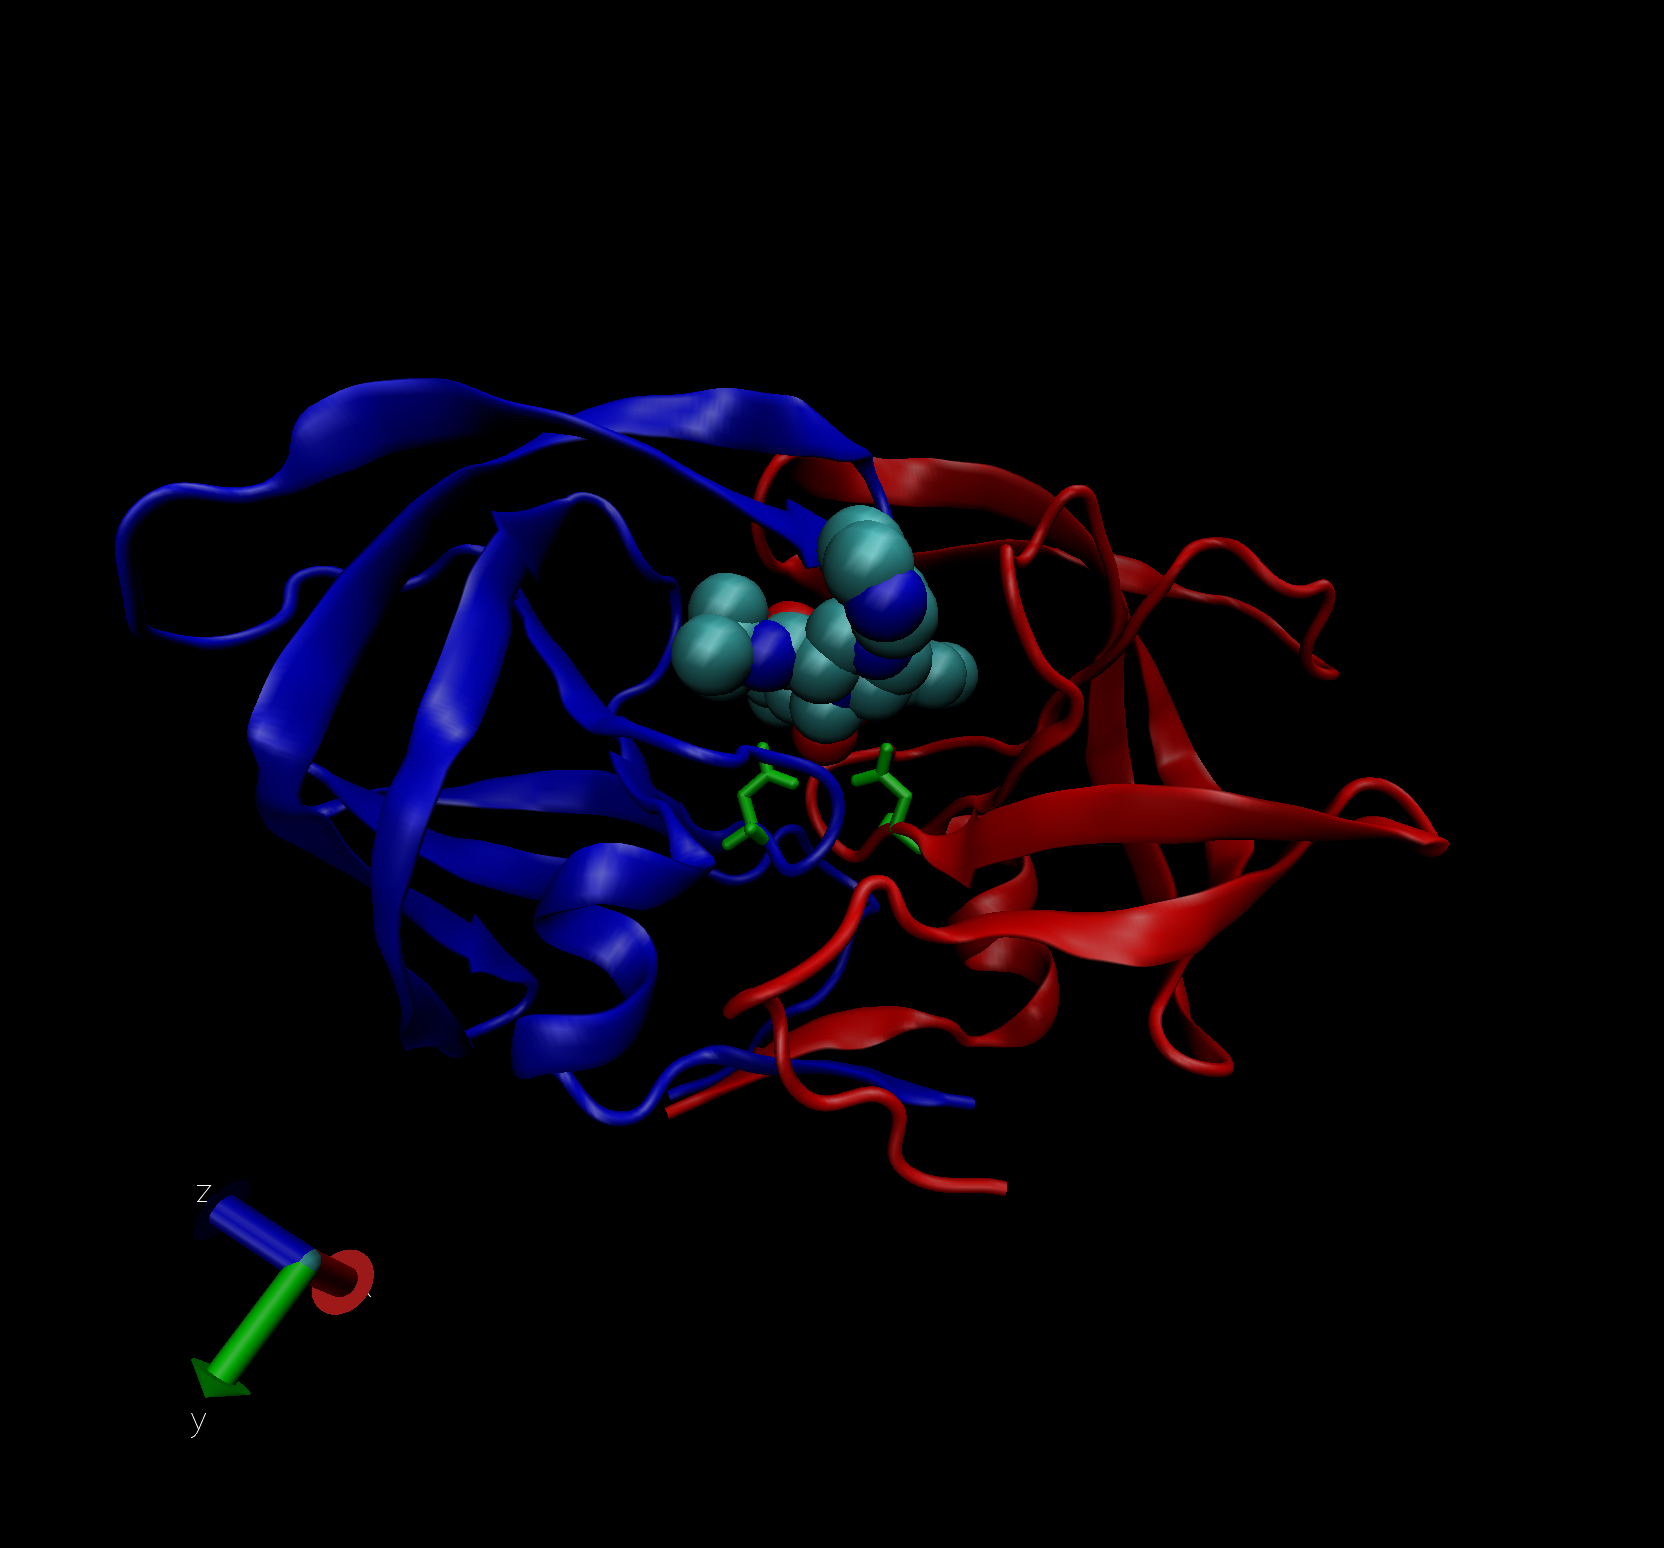
\includegraphics{my_structure.png}

\end{document}
